\part*{Analisis y recomendaciones}

\section{Resultados}

% TODO: Explicar que hicimos 100 corridas
% TODO: Explicar los rotulos de los graficos (price_hours-0 y eso)

\begin{figure}[H]

\begin{center}
    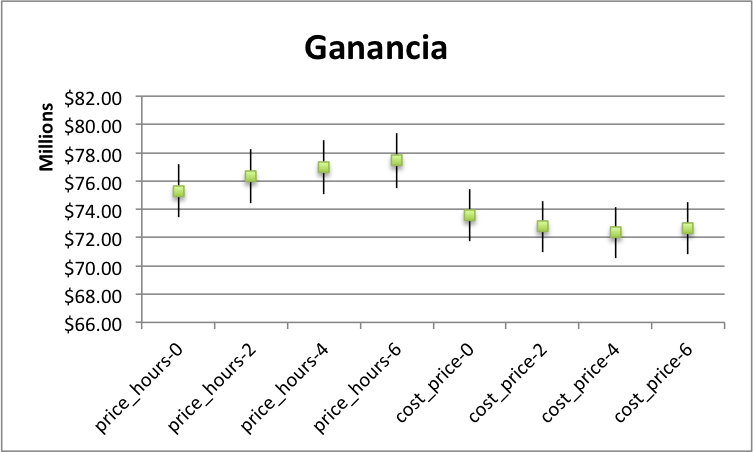
\includegraphics[width=0.75\textwidth,height=0.75\textheight,keepaspectratio]{./images/objective-earnings.png}
\end{center}

\label{fig:objective-earnings}
\caption{Ganancia con un intervalo del $5\%$ y $99\%$ de confianza}

\end{figure}

\begin{figure}[H]

\begin{center}
    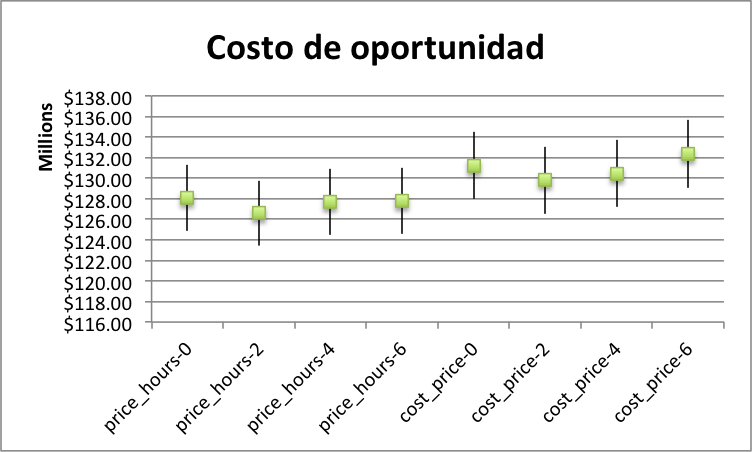
\includegraphics[width=0.75\textwidth,height=0.75\textheight,keepaspectratio]{./images/objective-cost.png}
\end{center}

\label{fig:objective-cost}
\caption{Costo de oportunidad con un intervalo del $5\%$ y $99\%$ de confianza}

\end{figure}

\begin{figure}[H]

\begin{center}
    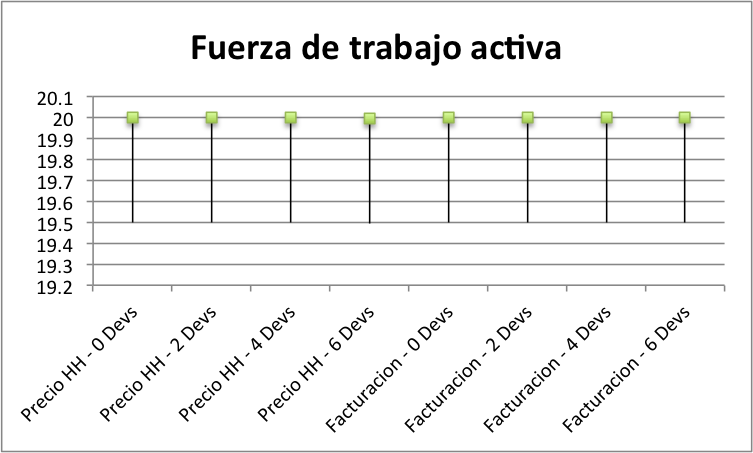
\includegraphics[width=0.75\textwidth,height=0.75\textheight,keepaspectratio]{./images/objetive-active-workforce.png}
\end{center}

\label{fig:objective-active-workforce}
\caption{Fuerza de trabajo activa con un intervalo del $5\%$ y $99\%$ de confianza}

\end{figure}

\section{????}

% TODO: Chamullar algo aca
